\documentclass[]{scrartcl}
\usepackage{tikz}

\begin{document}
	
\section{Dibujando en horizontalmente}

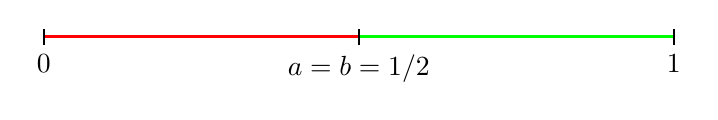
\begin{tikzpicture}[xscale=8]
\draw[-][draw=red, very thick] (0,0) -- (.5,0);
\draw[-][draw=green, very thick] (.5,0) -- (1,0);
\draw [thick] (0,-.1) node[below]{0} -- (0,0.1);
\draw [thick] (0.5,-.1) node[below]{$a=b=1/2$} -- (0.5,0.1);
\draw [thick] (1,-.1) node[below]{1} -- (1,0.1);
\end{tikzpicture}

\section{Dibujando en vertical}

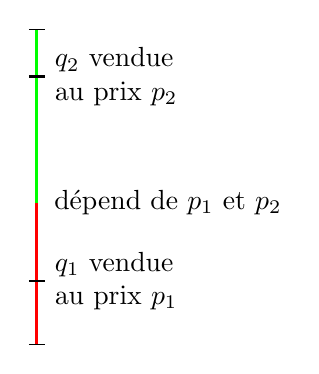
\begin{tikzpicture}[yscale=4]
\draw[-][draw=red, very thick] (0,0) -- (0,.45);
\draw[-][draw=green, very thick] (0,.45) -- (0,1);
\draw [thick] (-0.1,0.2) -- (0.1,.2) node[align=left, right]
{$q_1$ vendue\\au prix $p_1$};
\node[right] at (0.1,.45) {d\'epend de $p_1$ et $p_2$};
\draw [thick] ((-0.1,0.85) -- (0.1,.85) node[align=left, right]
{$q_2$ vendue\\ au prix $p_2$};
\draw (-0.1,0) -- (0.1,0);
\draw (-0.1,1) -- (0.1,1);
\end{tikzpicture}

\section{Dibujando curvas}

\begin{center}
	\begin{tikzpicture}
	\draw[<->] (6,0) node[below]{$q$} -- (0,0) --
	(0,6) node[left]{$V(q)$};
	\draw[very thick] (0,0) to [out=90,in=145] (5,4.5);
	\end{tikzpicture}
\end{center}

\section{Teniendo en cuenta tangencias}

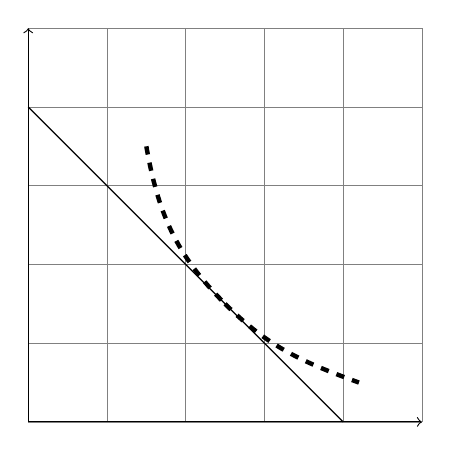
\begin{tikzpicture}
\draw [help lines] (0,0) grid (5,5);
\draw [<->] (5,0) -- (0,0) -- (0,5);
\draw (4,0) -- (0,4);
\draw[dashed,ultra thick]
(1.5,3.5) to [out=-80,in=135] (2.5,1.5);
\draw [dashed,ultra thick]
(2.5,1.5) to [out=-45,in=160] (4.2,0.5);
\end{tikzpicture}

\section{Otros ejemplos varios}

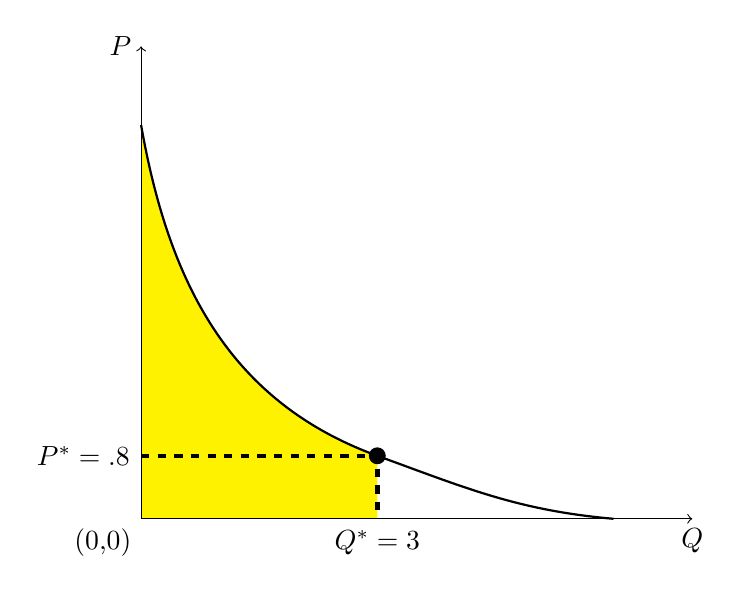
\begin{tikzpicture}
\path [fill=yellow] (0,0) -- (0,5) to [out=-80, in=160]
(3,.8) -- (3,0) -- (0,0);
\draw [<->] (0,6) node [left] {$P$} -- (0,0)
node [below left] {(0,0)} -- (7,0) node [below] {$Q$};
\draw [ultra thick, dashed] (0,.8) node [left] {$P^*=.8$} -- (3,.8)
-- (3,0) node [below] {$Q^*=3$};
\draw [fill] (3,.8) circle [radius=.1];
\draw [thick] (0,5) to [out=-80, in=160] (3,.8) to
[out=-20, in=175] (6,0);
\end{tikzpicture}

\section{Dibujando muchas curvas}

\begin{center}
	\begin{tikzpicture}[domain=0:0.5,xscale=13,yscale=3.8]
	\draw[<->] (0,2) node[left]{EUR}-- (0,0) -- (.7,0) node[below] {$q$};
	\draw[red] plot (\x, {0.25+\x/2+\x*\x/2}) node[right] {$v_1(x)$};
	\draw[green] plot (\x, {0.025+\x+\x*\x}) node[right] {$v_2(x)$};
	\draw[thin, dashed] plot (\x, {0.275+1.5*\x+1.5*\x*\x}) ;
	\draw[thick,domain=0:0.33666] plot (\x, {0.05+2*\x+2*\x*\x}) ;
	\draw[thick,domain=0.33666:0.5]
	plot (\x, {0.5+\x+\x*\x}) node[right] {$2\min[v_1,v_2]$};
	\end{tikzpicture}
\end{center}

\end{document}
